\section{Связь метода складного ножа и бутстрепа}

Что лучше, бутстреп или складной нож? Поскольку для этого требуется вычисление $\hat{\theta}$ только для $n$ наборов данных складного ножа, складной нож будет легче вычислить, если $n$ будет меньше, чем, скажем, $100$ или $200$ репликаций, используемых бутстрепом для оценки стандартной ошибки. Однако, рассматривая только $n$ выборок складного ножа, складной нож использует только ограниченную информацию о статистике $\hat{\theta}$, и, таким образом, можно предположить, что складной нож менее эффективен, чем бутстреп. Фактически оказывается, что складной нож можно рассматривать как приближение к бутстрепу. Это объясняется в задачах 11.4 и 11.5 и в главе 20. Вот суть идеи: рассмотрим линейную статистику, то есть статистику, которую можно записать в виде
\begin{equation}\label{eq11.17}
    \hat{\theta} = s(x) = \mu + \frac{1}{n}\sum\limits_{1}^{n}\alpha(x_{i}),
\end{equation}
где $\mu$ --- константа, а $\alpha(\cdot)$ --- функция. Среднее --- это простой пример линейной статистики, для которой $\mu = 0$ и $\alpha(x_i) = x_i$. Теперь для такой статистики, оказывается, что оценка по методу складного ножа и бутстреп оценка стандартных ошибок совпадают, за исключением незначительного множителя $\left\{(n-1)n\right\}^{1/2}$, используемого в определении складного ножа. Это именно то, что мы нашли для $\hat{\theta} = \Bar{x}$: складной нож дает оценку стандартной ошибки $\left\{\sum\limits_{1}^{n}(x_{i} - \Bar{x})^2/\{(n-1)n\}\right\}^{1/2}$ в то время как бутстреп приводит к этому значению, умноженному на $\left\{(n-1)n\right\}^{1/2}$. Неудивительно, что для линейной статистики нет потери информации при использовании складного ножа, поскольку знание линейной статистики для $n$ наборов данных складного ножа $x_{(i)}$ определяет значение $\hat{\theta}$ для любого бутстреп набора данных $x^{*}$ (задача 11.3).

При нелинейной статистике происходит потеря информации. Складной нож линейно аппроксимирует бутстреп: то есть он согласуется с бутстрепом (за исключением множителя $\left\{(n-1)n\right\}^{1/2}$) для некоторой линейной статистики вида \ref{eq11.17}, которая приближает $\hat{\theta}$. Детали этой интересной взаимосвязи приведены в задачах 11.5 и 11.6 и в главе 20. С практической точки зрения, эти результаты показывают, что точность оценки стандартной ошибки по методу складного ножа зависит от того, насколько $\hat{\theta}$ близка к линейности. Для сильно нелинейных функций складной нож может быть неэффективным, а иногда и опасным.

На рисунке 11.2 показаны результаты исследования этой неэффективности на конкретном примере. Мы сгенерировали $200$ выборок размером $10$ из двумерной нормальной совокупности с нулевым средним, единичной дисперсией и корреляцией $0.7$. Ящики с усами слева показывают оценки, полученные по методам бутстреп и складного ножа, стандартной ошибки для $\hat{\theta} = \Bar{x}$, а справа --- для коэффициента корреляции. Горизонтальные линии показывают истинную стандартную ошибку $\hat{\theta}$ в каждом случае. В обоих случаях бутстреп и складной нож демонстрируют небольшое смещение при оценке стандартной ошибки. Вариабельность оценки складного ножа немного больше, чем у бутстрепа для среднего (линейная статистика), но значительно больше для коэффициента корреляции (нелинейная статистика). По этой причине в последнем случае предпочтительнее использовать бутстреп. Задача 11.13 рассматривает бутстреп и  метод складного ножа для другой нелинейной статистики.

\noindent
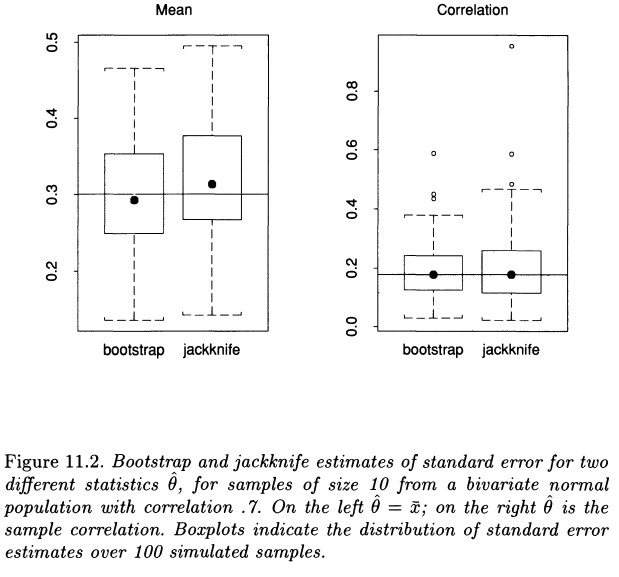
\includegraphics[width=\linewidth]{11/f11.2.png}
\newline

Точно так же можно показать, что оценка смещения складного ножа является приближением к начальной оценке смещения. Приближение в терминах квадратичной (а не линейной) статистики, которая имеет вид
\begin{equation}\label{eq11.18}
    \hat{\theta} = s(x) = \mu + \frac{1}{n}\sum\limits_{1 \leq i \leq n}\alpha(x_i) + \frac{1}{n^2}\sum\limits_{1 \leq i < j \leq n}\beta(x_i, x_j).
\end{equation}
Простым примером квадратичной статистики является выборочная дисперсия \ref{eq11.11}. Раскрывая ее, мы обнаруживаем, что ее можно выразить в форме уравнения \ref{eq11.18} (задача 11.9). Для такой статистики, если мы знаем значение $\hat{\theta}$ для $x$, а также $x_{(i)}, i = 1,2, \dots, n$, мы можем вывести значение $\hat{\theta}$ для любого бутстреп набора данных. Как показано в задачах 11.10–11.11, оценки смещения складного ножа и бутстрепа по существу совпадают для квадратичной статистики.